\documentclass[unknownkeysallowed]{beamer}

\usepackage[utf8]{inputenc}
\usepackage{graphicx}
\usepackage{epsfig}
\usepackage{hyperref}
\usepackage{booktabs, caption}
\usepackage{color}
\usepackage{tikz}


\beamertemplatenavigationsymbolsempty

\mode<presentation>
{
  \usetheme{sebslides}
  \setbeamertemplate{items}[circle]
}

\definecolor{uipoppy}{RGB}{225, 64, 5}
\definecolor{tumblue}{RGB}{0,100,188}
\definecolor{uipaleblue}{RGB}{96,123,139}
\definecolor{uiblack}{RGB}{0, 0, 0}

\newcommand{\topline}{%
  \tikz[remember picture,overlay] {%
    \draw[line width=0.35mm, uipaleblue]
    ([yshift=-1.2cm]current page.north west)
    -- ([yshift=-1.2cm,xshift=\paperwidth]current page.north west);}}

\title{Data Mining with Spare Grids}
\subtitle{Seminar: Computational Aspects of Machine Learning}
\author{Sebastian Kreisel}
\date{\today}

\begin{document}

{
\setbeamertemplate{footline}{}
\begin{frame}
  \maketitle
  \vspace{15px}
  \begin{center}
    \color{tumblue}{\footnotesize{Technische Universität München}}\\
    \vspace{6px}
    \includegraphics[width=1cm]{tum}
  \end{center}
\end{frame}
}
\addtocounter{framenumber}{-1}

\begin{frame}
  \frametitle{Overview}
  \topline
  \vspace{-10px}
  \begin{itemize}
    \item Motivation for Sparse Grids
      \vspace{8px}
    \item Sparse Grids: Basics
      \vspace{8px}
    \item Sparse Grids: Machine Learning
      \vspace{8px}
    \item Examples with Data Sets
      \vspace{8px}
    \item Parallelization and Implementation
  \end{itemize}
\end{frame}

\begin{frame}
  \frametitle{Motivation for Sparse Grids}
  \topline
  \vspace{-10px}
  \begin{block}{Grid based approaches in ML}
    \begin{itemize}
      \item Discretizes the space into a grid
      \item Basis--functions around grid points, not data points
    \end{itemize}

    \begin{figure}[!htb]
      \setbeamertemplate{caption}{\raggedright\insertcaption\par}
      \setbeamerfont{caption}{size=\footnotesize}
      \minipage{0.45\textwidth}
      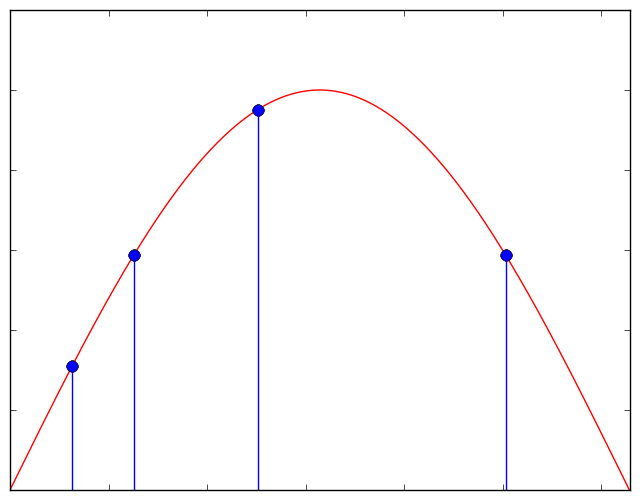
\includegraphics[width=\linewidth]{images/pointbase.png}
      \vspace{-12px}
      \caption{Point based}
      \endminipage
      \hspace{0.025\textwidth}
      \minipage{0.45\textwidth}
      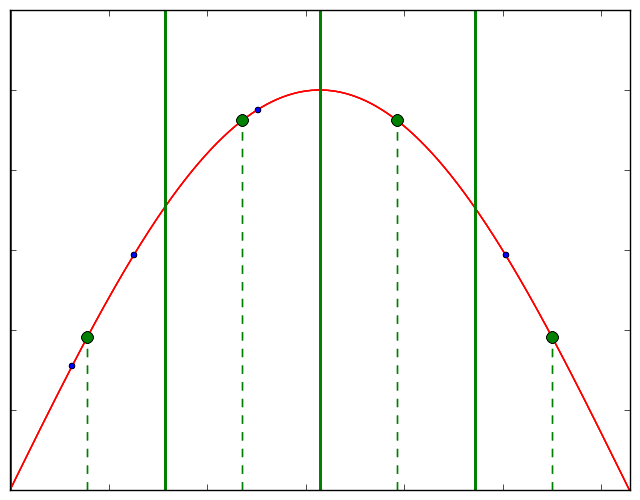
\includegraphics[width=\linewidth]{images/gridbase.png}
      \vspace{-12px}
      \caption{Grid based}
      \endminipage
    \end{figure}

  \end{block}

\end{frame}

\begin{frame}
  \frametitle{Motivation for Sparse Grids}
  \topline
  \vspace{-10px}
  \begin{block}{Suitable for}
    \begin{itemize}
      \item Big datasets
      \item Easily/automatically classifiable data
      \item Medical, seismic, commercial data
    \end{itemize}
  \end{block}
  \begin{block}{Curse of dimensionality}
    \begin{itemize}
    \item The volume of a space is exponential in it's dimensions
    \item The amount of training data required becomes unmanageable
      \begin{itemize}
      \item because of lacking computational/storage capacities
      \item because data aquesition is expensive
      \end{itemize}
    \item Becomes relevant for $d > 3$
    \item \textbf{Applies to full-grid discretization}
    \end{itemize}
  \end{block}
\end{frame}

\begin{frame}
  \frametitle{Full Grid Discretization}
  \topline
  \vspace{-10px}
  \begin{block}{1. A function to interpolate}
    \begin{figure}[!htp]

      \setbeamertemplate{caption}{\raggedright\insertcaption\par}
      \setbeamerfont{caption}{size=\footnotesize}
      \centering
      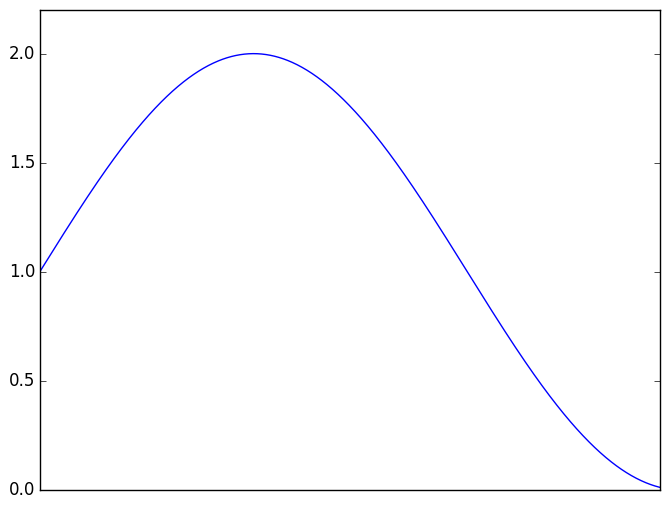
\includegraphics[width=7.5cm]{images/singlebasis_1}
      \vspace{-12px}
      \caption{$f(x) = sin(\pi \cdot x)$}
    \end{figure}
  \end{block}
\end{frame}
\begin{frame}
  \frametitle{Full Grid Discretization}
  \topline
  \vspace{-10px}
  \begin{block}{2. A (full, regular) grid}
    \begin{figure}[!htp]

      \setbeamertemplate{caption}{\raggedright\insertcaption\par}
      \setbeamerfont{caption}{size=\footnotesize}
      \centering
      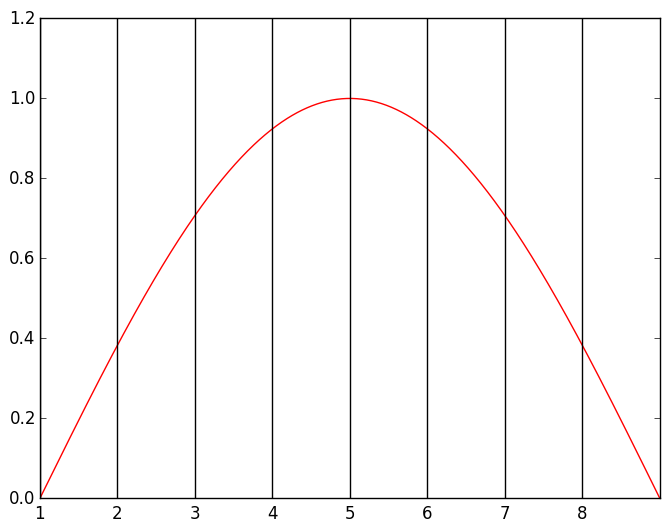
\includegraphics[width=7.5cm]{images/singlebasis_2}
      \vspace{-12px}
      \caption{Eight centered gridpoints $i \in \{1..8\}$}
    \end{figure}
  \end{block}
\end{frame}
\begin{frame}
  \frametitle{Full Grid Discretization}
  \topline
  \vspace{-10px}
  \begin{block}{3. A basis function (standard hat function)}
    \begin{figure}[!htp]

      \setbeamertemplate{caption}{\raggedright\insertcaption\par}
      \setbeamerfont{caption}{size=\footnotesize}
      \centering
      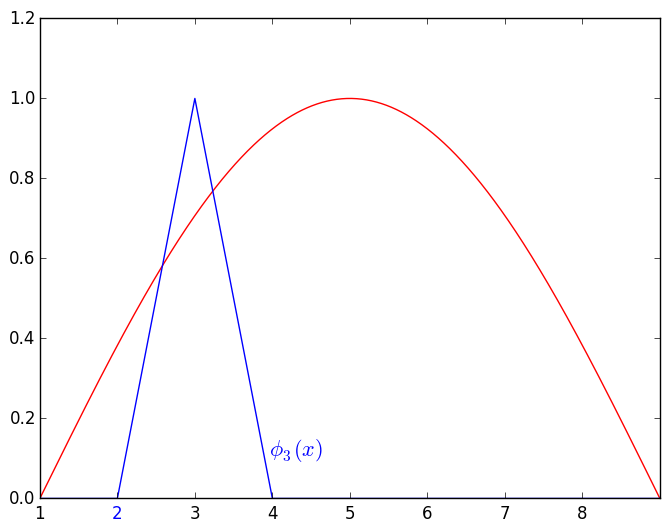
\includegraphics[width=7.5cm]{images/singlebasis_3}
      \vspace{-12px}
      \caption{$\phi(x - 3)$ with $\phi(x) = \text{max}(abs(1 - x), 0)$}
    \end{figure}
  \end{block}
\end{frame}
\begin{frame}
  \frametitle{Full Grid Discretization}
  \topline
  \vspace{-10px}
  \begin{block}{4. A Coefficient (Surplus)}
    \begin{figure}[!htp]

      \setbeamertemplate{caption}{\raggedright\insertcaption\par}
      \setbeamerfont{caption}{size=\footnotesize}
      \centering
      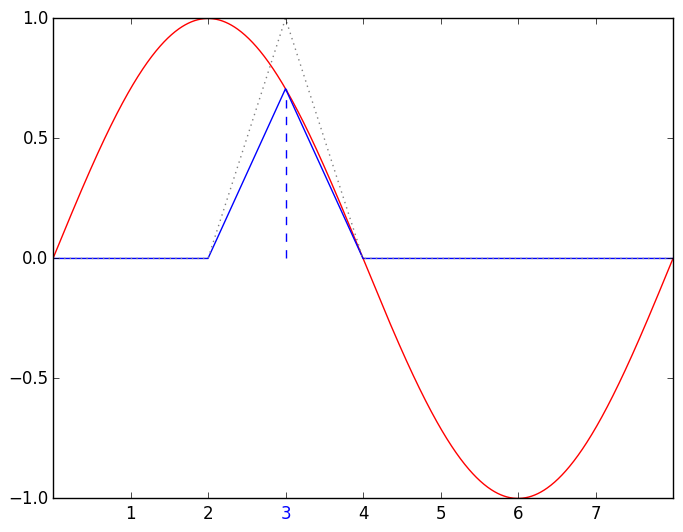
\includegraphics[width=7.5cm]{images/singlebasis_4}
      \vspace{-12px}
      \caption{$\alpha_2 \cdot \phi_2(x)$}
    \end{figure}
  \end{block}
\end{frame}
\begin{frame}
  \frametitle{Full Grid Discretization}
  \topline
  \vspace{-10px}
  \begin{block}{Sum over all basis functions}
    \begin{figure}[!htp]

      \setbeamertemplate{caption}{\raggedright\insertcaption\par}
      \setbeamerfont{caption}{size=\footnotesize}
      \centering
      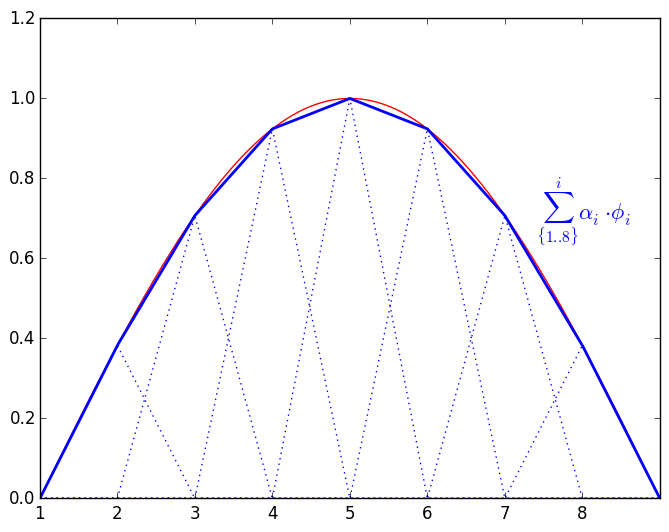
\includegraphics[width=7.5cm]{images/singlebasis_5}
      \vspace{-12px}
      \caption{$f(x) \approx \hat{f}(x) = \sum_i{\alpha_i \cdot \phi_i}$}
    \end{figure}
  \end{block}
\end{frame}
\begin{frame}
  \frametitle{Full Grid Discretization}
  \topline
  \vspace{-10px}
  \begin{block}{Full grid interpolation in one dimension}
    \setbeamertemplate{enumerate items}[default]
    \begin{enumerate}
    \item A function $f(x)$
    \item Gridpoints indexed by $i \in \{1,2,\dots\}$
    \item Basis/Ansatz functions; i.e. hat function $\phi_i(x)=\text{max}(1 - |x|, 0)$
    \item Coefficients $\alpha_i$ (hierachcial surplusses)
    \end{enumerate}
    \vspace{10px}
    \begin{center}
      $f(x) \approx$ $\hat{f}(x) = \sum_{i}^{}{\alpha_i \phi_i(x)}$
    \end{center}
  \end{block}
\end{frame}

\begin{frame}
  \frametitle{Full Grid Discretization}
  \topline
  \vspace{-10px}
  \begin{block}{Level of detail}
    \begin{itemize}
    \item Level $l \in \{1,2,\dots\}$ in addition to index $i \in 2^l$
    \end{itemize}
  \end{block}
  \begin{block}{$D$ dimensions}
    \begin{itemize}
    \item For each dimension $d$: $\hat{f}_d$
    \item Tensor product over all dimensions $\hat{f}(x) = \prod_j{ \hat{f}_j(x) }$
    \end{itemize}
  \end{block}
\end{frame}

\begin{frame}
  \frametitle{Sparse Grids -- Basics}
  \topline
  \vspace{-10px}
  \begin{block}{Hirachial Basis}
    \begin{itemize}
    \item Grouping gridpoints into levels $l_1, l_2,\dots$
    \item For each level a set of gridpoints $I_l = \{ \ i \ \ | \ \ 1 < i < 2^l - 1; \ \ i \text{ odd }\}$
      \begin{itemize}
      \item $I_1 = \{1\}$
      \item $I_2 = \{1, 3\}$
      \item $I_3 = \{1, 3, 5, 7\}$
      \item $\ \dots$
      \end{itemize}
    \item For all dimensions seperately
    \end{itemize}
  \end{block}
  \begin{center}
    $\hat{f_d}(x) = \sum_{l,i}{ \ \alpha_{l,i} \ \cdot \ \phi_{l,i}(x)}$
  \end{center}
\end{frame}

\end{document}
